\cleartooddpage[\thispagestyle{empty}]
\chapter{Cerebral Vasculature and the Impact of Disturbed Flow}\label{CHAPTER2}
The human vasculature is a system aimed at carrying blood and lymph through the body. The arteries of the vascular system help deliver oxygenated blood, nutrients, and components such as inflammatory markers and hormones through the body, while the veinous structures help take cellular and tissue waste matter to organs such as the lungs, liver and kidneys for removal as well as carrying deoxygentaed blood back to the heart. The lympahtic vessels carry lymph (fluid containing water and blood cells) to help maintain hemodynamic pressures withing the body. Intracranial aneurysms have only been shown to develop within the arterial portion of the vasculature, and as such will be the the part of the vascualture fouced upon in this work. The innermost layer of arteries, known as the tunica intima, is made of a monolayer of endothelial cells (EC) supported by a layer of collagen and elastin. This intimal layer comes into direct contact with the hemodynamic flow environment of the lumen (hollow cavity of the arterial system in which blood flows). This endothelial layer serves multiple purposes: hemodynamic mechanosensors, reacting to fluid forces and transducing said force into biochemical signals triggering cellular cascades controlling vascular tone and homeostasis\cite{dorland2017cell,cancel2016endothelial,chien2007mechanotransduction}, and acting as a selective permeability layer for macromolecules\cite{benn2016ve,ghim2017visualization,mundi2018endothelial}. Underlying the intima layer is the the tunica media, or media, a layer composed of smooth muscle cells, elastic connective tissue and collagen fibers. The main purpose of the media layer is to contract or dilate the arterial vasculature in response to (as signaled by the intima layer) differing hemodynamic conditions as a means to regulate circulation within the body\cite{bogunovic2019impaired,michel2018genetics}. The outermost layer of arteries, the tunica externa/adventitia, is composed of collagen fibers and elastic tissue helping to maintain the mechanical properties of the vasculature, while the collagen having a secondary purpose of anchoring the vessel to surrounding tissues (improving vessel stability)(Fig.~\ref{Vasculature_Layers}).

\begin{figure}[!h]
  \begin{center}
    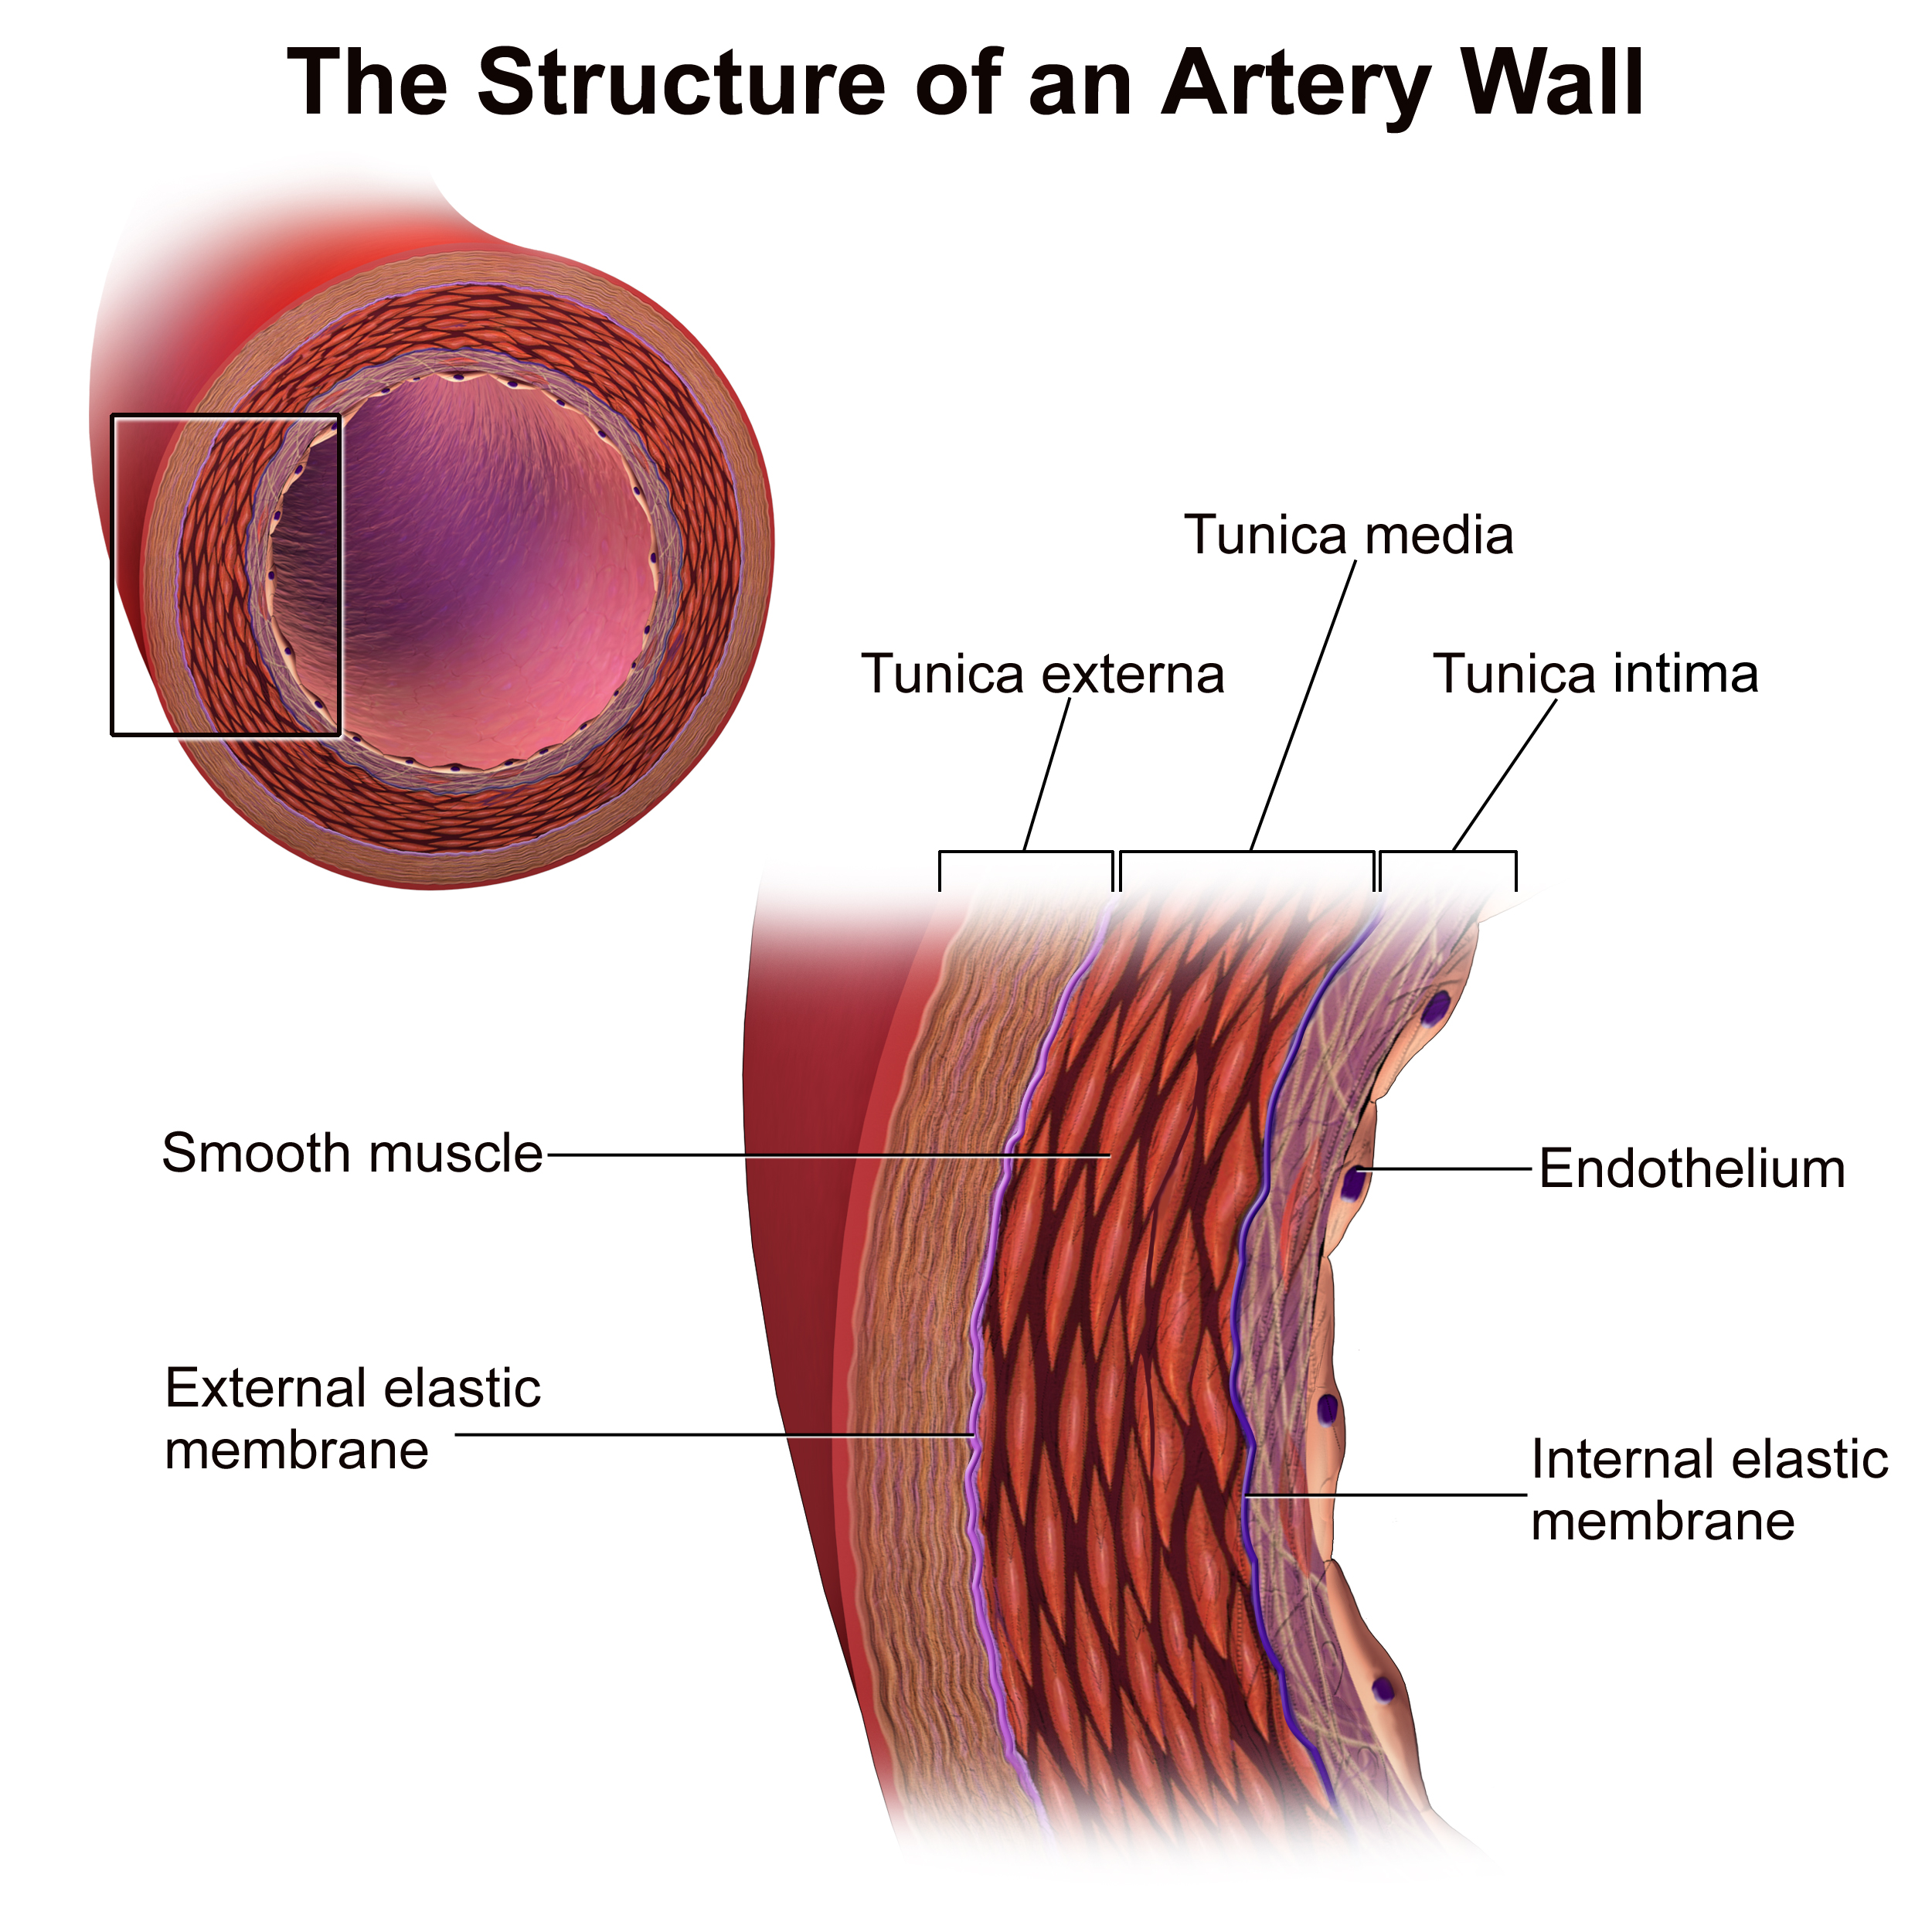
\includegraphics[width=3.5in]{Vasculature}
  \end{center}
  \caption{Layers of the vasculature. Original image from \cite{WIKI_Vessel}}
  \label{Vasculature_Layers}
\end{figure}

Docendi eligendi sit et, pri ea dicam eligendi percipitur, has soleat 
dolores convenire te. Sed altera placerat an, id verterem abhorreant 
interesset mea. Eum at ceteros efficiantur. Eos id voluptaria efficiendi 
comprehensam. 

In mel modo dicam vocibus, eruditi consectetuer vim no, cu quaestio 
instructior eum. Justo nostrud fuisset ea mea, eam an libris repudiandae 
vituperatoribus. Est choro corrumpit definitionem at. Vel sint adhuc vocibus 
ea, illud epicuri eos no. Sea simul officiis ea, et qui veri invidunt 
appellantur. Vix et eros ancillae pertinax.

Aliquip lobortis ei est, at error viris graeco sed. Vel te elitr detracto, 
modo graecis scripserit ex nec. Errem utamur viderer per no, eam ea eripuit 
referrentur. Pro te dicat disputando. 

\vspace{0.25in}
\begin{table}[hbt]
  \caption{A portrait table:
    first column represents the year in which the Nobel prize in
    physics was awarded; second column indicates the name of the
    scientist and the third column is the work for which the Nobel
    prize was awareded}
  \begin{center}
    \begin{tabular}{lll}
      \hline
      \multicolumn{1}{c}{\textbf{Year}} & 
      \multicolumn{1}{c}{\textbf{Scientist(s)}} &
      \multicolumn{1}{c}{\textbf{Nobel Work}}\\
      \hline
      1901 & W. C. R\"{o}ntgen & X-rays\\
      1902 & H. A. Lorentz & Influence of magnetism on radiation\\
           & P. Zeeman     & Influence of magnetism on radiation\\
      1903 & A. H. Becquerel & Spontaneous radioactivity\\
           & M. Curie        & Radiation phenomena discovered by Becquerel\\
           & P. Curie        & Radiation phenomena discovered by Becquerel\\
      1904 & J. W. Strutt & Argon\\
      1905 & P. E. A. von Lenard & Cathode rays\\
      1906 & J. J. Thomson & Electrical conductivity of gases\\
      1907 & A. A. Michelson & Spectroscopic and metrological investigations\\
      1908 & G. Lippmann & Photographic reproduction of colours\\
      1909 & K. F. Braun & Wireless telegraphy\\
           & G. Marconi &  Wireless telegraphy\\
      1910 & J. D. van der Waals & Equation of state of gases and liquids\\
      1911 & W. Wien & Laws governing heat radiation\\
      1912 & N. G. Dal\`{e}n & Automatic regulators for lighting coastal beacons\\
           &                 & and light buoys\\
      \hline
    \end{tabular}
    \label{CHAPTER2_TABLE01}
  \end{center}
\end{table}

As explained in Table \ref{CHAPTER2_TABLE01},
Ex offendit elaboraret cum has ex natum honestatis, impedit similique ex duo. 
Et mei mollis scripta, et vim labores phaedrum, in cum facete saperet. 
Splendide elaboraret comprehensam qui ne. Putant verterem no vim, mea solum 
veritus definitiones ei, no labitur propriae deseruisse est. Ius illud everti 
salutandi id, eu facer pericula principes est.

\begin{figure}[htb]
  \begin{center}
    \begin{tikzpicture}[
      thick,
      >=stealth',
      dot/.style = {
        draw,
        fill = white,
        circle,
        inner sep = 0pt,
        minimum size = 4pt
      }
      ]
      \coordinate (O) at (0,0);
      \draw[->] (-0.3,0) -- (8,0) coordinate[label = {below:$x$}] (xmax);
      \draw[->] (0,-0.3) -- (0,5) coordinate[label = {right:$f(x)$}] (ymax);
      \path[name path=x] (0.3,0.5) -- (6.7,4.7);
      \path[name path=y] plot[smooth] coordinates {(-0.3,2) (2,1.5) (4,2.8) (6,5)};
      \scope[name intersections = {of = x and y, name = i}]
        \fill[gray!20] (i-1) -- (i-2 |- i-1) -- (i-2) -- cycle;
        \draw (0.3,0.5) -- (6.7,4.7) node[pos=0.8, below right] {secant};
        \draw[red] plot[smooth] coordinates {(-0.3,2) (2,1.5) (4,2.8) (6,5)};
        \draw (i-1) node[dot, label = {above:$P$}] (i-1) {} -- node[left]
          {$f(x_0)$} (i-1 |- O) node[dot, label = {below:$x_0$}] {};
        \path (i-2) node[dot, label = {above:$Q$}] (i-2) {} -- (i-2 |- i-1)
          node[dot] (i-12) {};
        \draw (i-12) -- (i-12 |- O) node[dot,
          label = {below:$x_0 + \varepsilon$}] {};
        \draw[blue, <->] (i-2) -- node[right] {$f(x_0 + \varepsilon) - f(x_0)$}
          (i-12);
        \draw[blue, <->] (i-1) -- node[below] {$\varepsilon$} (i-12);
        \path (i-1 |- O) -- node[below] {$\varepsilon$} (i-2 |- O);
        \draw[gray] (i-2) -- (i-2 -| xmax);
        \draw[gray, <->] ([xshift = -0.5cm]i-2 -| xmax) -- node[fill = white]
          {$f(x_0 + \varepsilon)$}  ([xshift = -0.5cm]xmax);
      \endscope
    \end{tikzpicture}
  \end{center}
  \caption{Fancy mathematical plots using TikZ package}
  \label{CHAPTER2_FIG02}
\end{figure}

Simul noster voluptaria eam ei, sint regione pri ei. Cum no utinam equidem, 
falli bonorum prodesset an qui. Alterum dissentiet vituperatoribus te eam, 
eos ea suas oblique. Per ea utinam facilisi. Per iudico probatus complectitur 
et, cum tollit atomorum rationibus ea.

Docendi eligendi sit et, pri ea dicam eligendi percipitur, has soleat 
dolores convenire te. Sed altera placerat an, id verterem abhorreant 
interesset mea. Eum at ceteros efficiantur. Eos id voluptaria efficiendi 
comprehensam.

Simul noster voluptaria eam ei, sint regione pri ei. Cum no utinam equidem, 
falli bonorum prodesset an qui. Alterum dissentiet vituperatoribus te eam, 
eos ea suas oblique. Per ea utinam facilisi. Per iudico probatus complectitur 
et, cum tollit atomorum rationibus ea.

\begin{figure}[htb]
  \begin{center}
    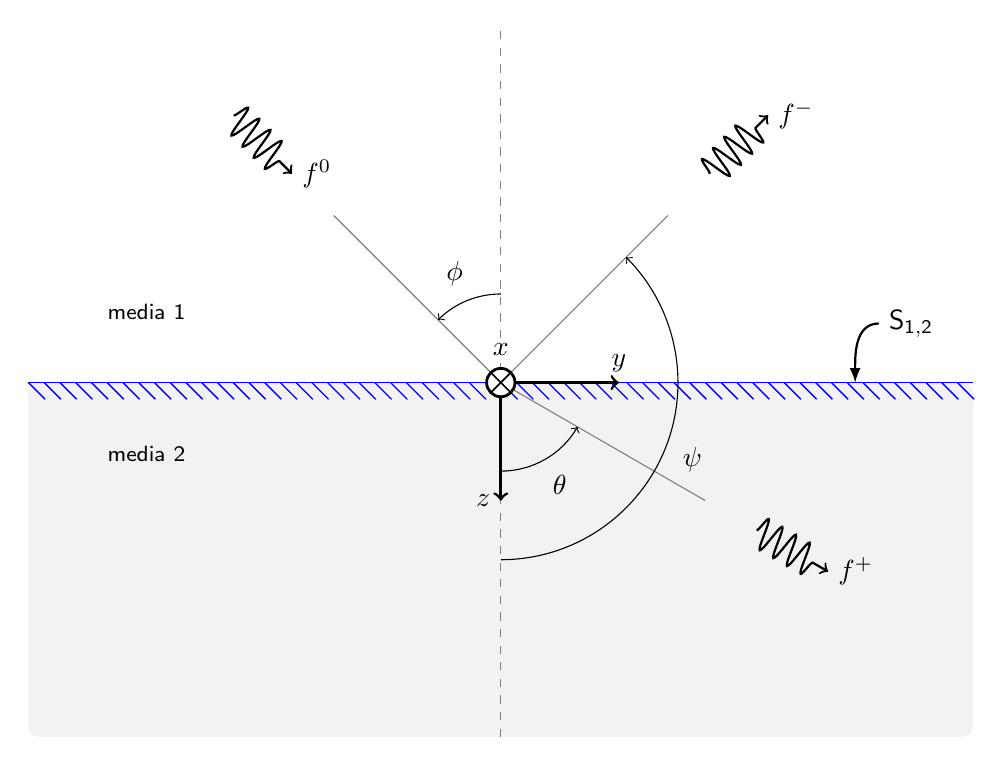
\begin{tikzpicture}[
      scale=1.5,
      media/.style={font={\footnotesize\sffamily}},
      wave/.style={
        decorate,decoration={snake,post length=1.4mm,amplitude=2mm,
        segment length=2mm},thick},
      interface/.style={
        % The border decoration is a path replacing decorator.
        % For the interface style we want to draw the original path.
        % The postaction option is therefore used to ensure that the
        % border decoration is drawn *after* the original path.
        postaction={draw,decorate,decoration={border,angle=-45,
                    amplitude=0.3cm,segment length=2mm}}},
      ]
      % Round rectangle
      \fill[gray!10,rounded corners] (-4,-3) rectangle (4,0);
      % Interface
      \draw[blue,line width=.5pt,interface](-4,0)--(4,0);
      % Vertical dashed line
      \draw[dashed,gray](0,-3)--(0,3);
      % Coordinates system
      \draw(0,0.15)node[above]{$x$};
      \draw[<->,line width=1pt] (1,0) node[above]{$y$}-|(0,-1) node[left]{$z$};
      % Incidence
      \draw[->,wave]
        (135:3.2cm)--(135:2.5cm)node[right]{$f^0$};
      \draw[gray](0:0cm)--(135:2cm);
      \path (0,0)++(113:1cm)node{$\phi$};
      \draw[->](0,0.75)arc(90:135:.75cm);
      % Transmission
      \draw[->,wave]
        (-30:2.5cm)--(-30:3.2cm)node[right]{$f^+$};
      \draw[gray](0:0cm)--(-30:2cm);
      \path (0,0)++(-60:1cm)node{$\theta$};
      \draw[->] (0,-0.75) arc (-90:-30:.75cm);
      % Reflection
      \draw[->,wave]
        (45:2.5cm)--(45:3.2cm)node[right]{$f^-$};
      \path (0,0)++(-22:1.75cm) node{$\psi$};
      \draw[gray](0:0cm)--(45:2cm);
      \draw[->] (0,-1.5)arc(-90:45:1.5cm);
      % Media names
      \path[media] (-3,.6)  node {media 1}
                   (-3,-.6) node {media 2};
      % $x$ axis
      \filldraw[fill=white,line width=1pt](0,0)circle(.12cm);
      \draw[line width=.6pt] (0,0)
        +(-135:.12cm) -- +(45:.12cm)
        +(-45:.12cm) -- +(135:.12cm);
      % Interface pointer
      \draw[-latex,thick](3.2,0.5)node[right]{$\mathsf{S_{1,2}}$}
        to[out=180,in=90] (3,0);
      % To-paths are really useful for drawing curved lines. The above
      % to path is equal to:
      %
      % \draw[-latex,thick](3.2,0.5)node[right]{$\mathsf{S_{1,2}}$}
      %      ..controls +(180:.2cm) and +(up:0.25cm) .. (3,0);
      % Internally the to path is translated to a similar bezier curve,
      % but the to path syntax hides the complexity from the user. 
    \end{tikzpicture}
  \end{center}
  \caption{Incidence, transmission and reflection}
  \label{CHAPTER2_FIG03}
\end{figure}

Docendi eligendi sit et, pri ea dicam eligendi percipitur, has soleat 
dolores convenire te. Sed altera placerat an, id verterem abhorreant 
interesset mea. Eum at ceteros efficiantur. Eos id voluptaria efficiendi 
comprehensam. Simul noster voluptaria eam ei, sint regione pri ei. Cum no 
utinam equidem, falli bonorum prodesset an qui. 
